%!TEX root = ../summary.tex

\section{From Source Code to Physical Deployment}

\subsection{Version Control Systems}
Versioning aims to control an manage all artifacts used and created in a process.
VCSes can be differentiated between local, centralized and distributed VCSes.
Local ones are kept only on the local systems where the artifacts are developed.
Centralized VCSes have a central server that holds the code base and single clients have only a single version of the artifacts available.
Distributed VCSes have different versions locally as well as on a central repository.

\subsubsection{SVN (central) vs Git (distributed)}
SVN stores information as a list of file-based changes.
Git on the other hand handles the data more like a set of snapshots of a miniature file system.
Every commit is a picture taken of what all files look like at that moment and pointers to these snapshots are stored.

\subsubsection{Git}
\paragraph{File States}
In Git, a file can have three different stages.
In the modified state the file has changes that are not yet committed to the local database.
In the staged state the file then has been marked to go into the next commit and in the committed state the data is safely stored in the local database.
In that state the data can be pushed to the remote repository.

\paragraph{Commands}
\begin{figure}[H]
  \centering
  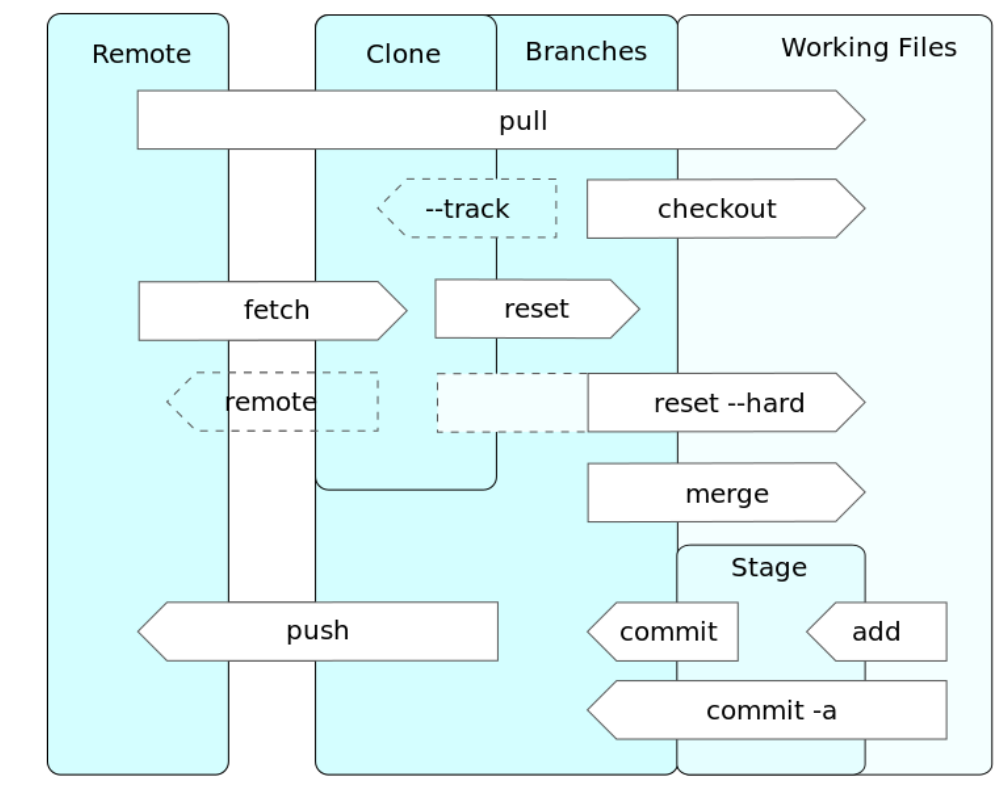
\includegraphics[width=.8\textwidth]{images/git_commands.png}
  \caption{Git Commands}
\end{figure}

\paragraph{Branching}
Git keeps snapshots of the commits named by hashes of the local files.
Branches are pointers to these commits.
The HEAD pointer points to the current local commit, the default branch is called master and adding a branch means adding a named pointer to a commit.

\subsection{Continuous Integration}
\begin{figure}[h]
  \centering
  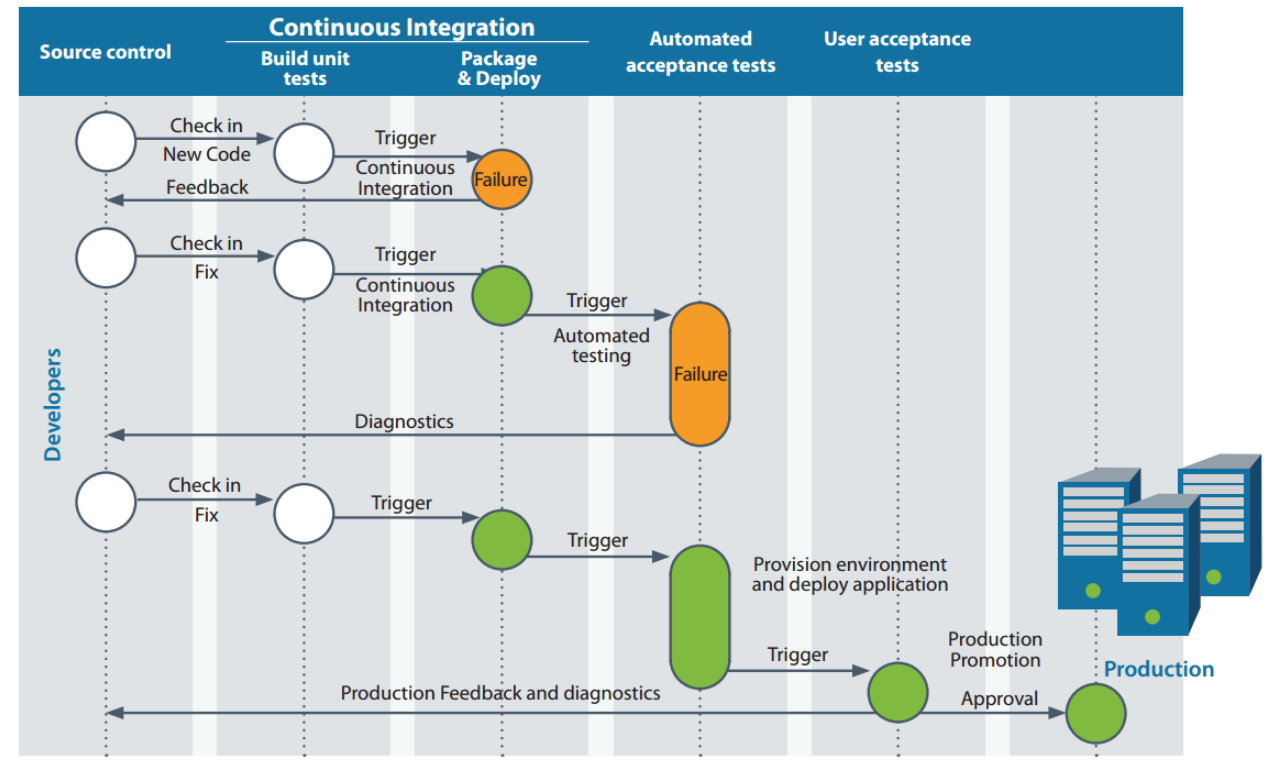
\includegraphics[width=.8\textwidth]{images/continuous_integration.png}
  \caption{Continuous Integration}\label{fig:continuous_integration}
\end{figure}
A development process (c.f.\ Figure~\ref{fig:continuous_integration}) with continuous integrations maintains a single source repository with an automated build and tests.
Every commit triggers a this automated procedures for what it is important to keep the build process fast.
Test should be executed in a clone of the production environment.
The automated build process makes it easy for everyone to get the latest executables and makes the result visible to everyone.
In the end, even the deployment can be automated potentially.\\

\textbf{Pros}
\begin{itemize}
  \item Reducing risk
  \item Integrated quality assurance
  \item Reports and feedback on the health of the code base
  \item Availability of a stable release
  \item Everyone commits to the main branch every day which results in modular, less complex code
\end{itemize}

